\documentclass[11pt]{article}
\input{commandPlotResults.tex}
\usepackage[frenchb,english]{babel}
\usepackage[margin=15mm]{geometry}
\usepackage{graphicx}
 \usepackage{color}
\usepackage{multirow}
\usepackage{multicol}
\usepackage{tikz}
\usepackage{adjustbox}
\usepackage{lscape}
\usepackage{float}
\usepackage{array}
\usepackage{calc}
\usepackage{amsmath}
\usepackage{dsfont}
\usepackage{hyperref}
\usepackage{tocloft}
\usepackage{titlesec}
\usepackage[scaled=.90]{helvet}
\usepackage{booktabs}
% Options pour les liens hypertexte
\hypersetup{
       backref=true,                           % Permet d'ajouter des liens dans
       pagebackref=true,                       % les bibliographies
       hyperindex=true,                        % Ajoute des liens dans les index.
       colorlinks=true,                        % Colorise les liens.
       breaklinks=true,                        % Permet le retour à la ligne dans les liens trop longs.
       urlcolor= black,                         % Couleur des hyperliens.
       linkcolor= black,                        % Couleur des liens internes.
       citecolor=black,			% Couleur pour les liens de biblio
       bookmarks=true,                         % Créé des signets pour Acrobat.
       bookmarksopen=true,                     % Si les signets Acrobat sont créés,
                                               % les afficher complètement.
       pdftitle={},  % Titre du document.
                                               % Informations apparaissant dans
       pdfauthor={Sebastien Benzekry},                      % dans les informations du document
       pdfsubject={Mathematics}           % sous Acrobat.
    }

\titleformat{\section}
  {\normalfont\sffamily\Large\bfseries}
  {\thesection}{0em}{}

\newcounter{fignb}  % to number supplementary figures 
\newcounter{tabnb} % to number supplementary tables
%-----------------------------------------------------------
%-----------------------------------------------------------
%-----------------------------------------------------------
\begin{document}
\renewcommand\thesection{}
\renewcommand\thesubsection{}
\renewcommand\thesubsubsection{}
\fontfamily{phv}\selectfont
\pagenumbering{gobble}
%-----------------------------------------------------------%%%
\graphicspath{
{/Users/benzekry/work/marseille/neuroblastome_andre/code/}
{figures_files/}
}
%-----------------------------------------------------------%%%
\setlength{\parindent}{0mm}
%-----------------------------------------------------------%%%
\textbf{\Huge{Figures and Tables}}

\renewcommand{\cfttoctitlefont}{\normalfont\MakeUppercase}
\renewcommand{\contentsname}{}
\tableofcontents

\vskip2cm
%-----------------------------------------------------------%%%
\newpage
\vskip2cm
\renewcommand\thesection{}
%-----------------------------------------------------------
\def\spaceV{\vskip0.5cm}
\pagenumbering{gobble}
%-----------------------------------------------------------
%-----------------------------------------------------------
\newpage
\stepcounter{tabnb}
\section{Table \arabic{tabnb}: Patients characteristics}
\spaceV
\begin{center}
\includegraphics[width=0.8\textwidth]{table_1.pdf}
\end{center}

%-----------------------------------------------------------
\newpage
\stepcounter{tabnb}
\section{Table \arabic{tabnb}: Multivariable Cox analysis of overall survival}
\spaceV
\begin{center}
\begin{tabular}{lrrrr}
\toprule
{} &  Hazard ratio &      p &  coef lower 95\% &  coef upper 95\% \\
covariate         &               &        &                  &                  \\
\midrule
age               &         0.997 &  0.739 &            0.979 &             1.02 \\
sex               &          1.15 &  0.771 &            0.457 &             2.88 \\
log(LDH)          &          2.57 & 0.0493 &                1 &             6.59 \\
SIOPEN            &          1.01 &  0.386 &            0.982 &             1.05 \\
MYCN              &         0.831 &  0.804 &            0.192 &             3.59 \\
tumor size        &             1 &  0.764 &            0.998 &                1 \\
$\log(\mu)$       &         0.884 &  0.183 &            0.737 &             1.06 \\
visible threshold &         0.997 &  0.487 &            0.987 &             1.01 \\
\bottomrule
\end{tabular}

\end{center}
%-----------------------------------------------------------
\newpage
\stepcounter{fignb}
\section{Figure \arabic{fignb}: Schematic of the mathematical model}
\spaceV
\begin{center}
\includegraphics[width=0.8\textwidth]{figure_1}
\end{center}
Primary and secondary tumors are assumed to have exponential growth kinetics governed by a proliferation rate $\alpha$. Dissemination of metastasis is controlled by the parameter $\mu$. From these and primary tumor size at diagnosis $S_d$, the primary tumor age $T_d$ can be computed and simulations of the natural history can be performed. Adjunction of a visibility threshold $S_{vis}$ results in predictions of the number of visible metastases $N_{vis}$ and total cancer mass (primary + secondary tumors) $S_p + M$. These are respectively compared to the SIOPEN score and lactate dehydrogenase level. The time of birth of the first metastasis is denoted $T_{fm}$ and the time to reach $S_{vis}$ from one cell $\tau_{vis}$. Note that the number of visible metastases at time $T_d$ is the total number of metastases at time $T_d - \tau_{vis}$.
%-----------------------------------------------------------
\newpage
\stepcounter{fignb}
\section{Figure \arabic{fignb}: Overall and progression-free survival}
\spaceV
\begin{center}
\includegraphics[width=0.6\textwidth]{statistical_analysis/OS_PFS}
\end{center}
Kaplan-Meier estimates of overall and progression-free survival. Dotted lines show survival rates at 3 years (PFS=48.1\%, OS=56.6\%) and 5 years (PFS=31.8\%, OS=38.2\%). Median PFS = 31 months, median OS = 43 months.
%-----------------------------------------------------------
\newpage
\stepcounter{fignb}
\section{Figure \arabic{fignb}: Descriptive power of the mathematical model}
\spaceV
\begin{center}
\includegraphics[width=1\textwidth]{figure_3}
\end{center}

A. Fit of the SIOPEN data. Solid line is the identity line.\\
B. Fit of the LDH data. Solid line is the identity line.\\
C. Correlation matrix of all features including clinical variables and (log) of the mathematical parameter $\mu$. Level of darkness indicates positive correlation whereas brightness indicates negative correlation

%-----------------------------------------------------------
\newpage
\stepcounter{fignb}
\section{Figure \arabic{fignb}: Mechanistic simulations of the pre-diagnosis history of high-risk neuroblastoma patients }
\spaceV
\begin{center}
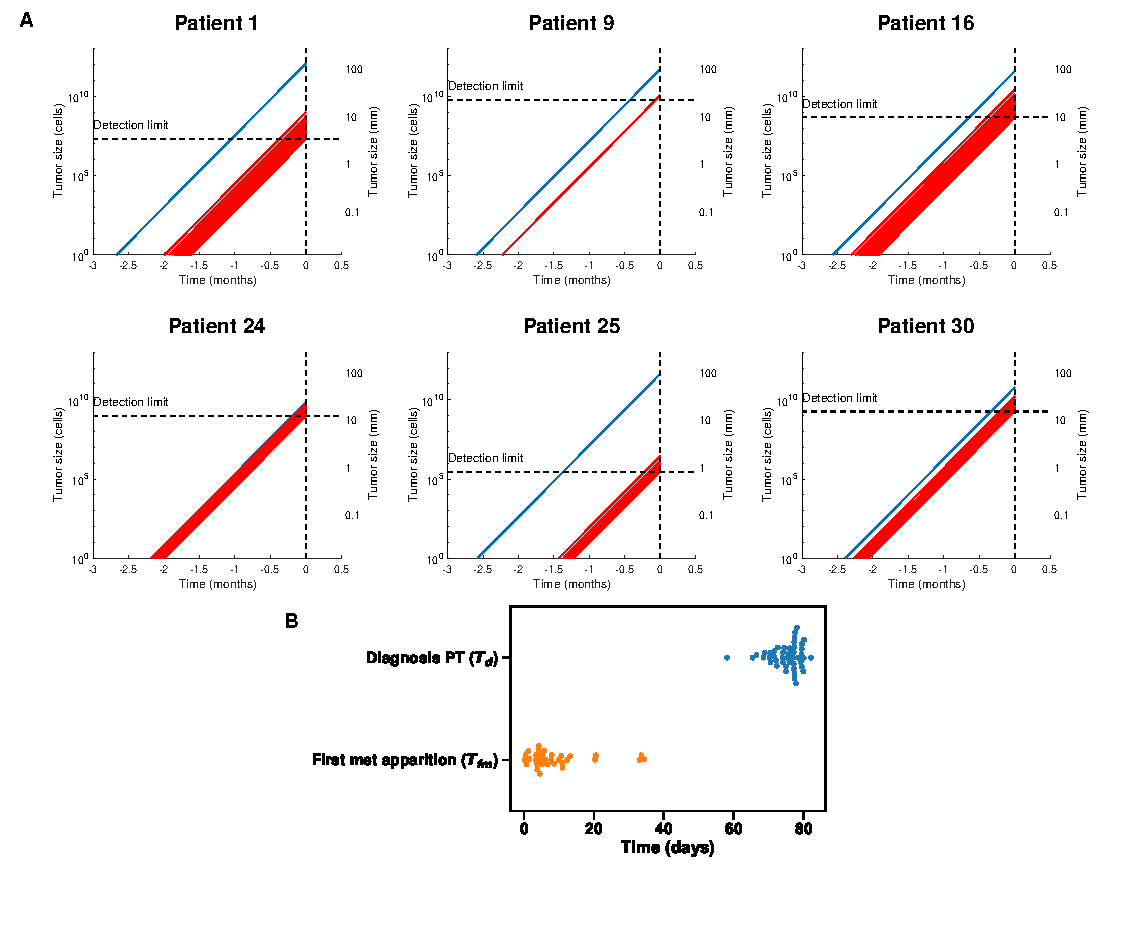
\includegraphics[width=1\textwidth]{figure_4}
\end{center}
A mechanistic model was calibrated using patient data of SIOPEN score (number of visible metastases) and LDH levels (total cancer burden), which resulted in individual values of the model parameters $\mu$ and $S_{vis}$. These values are reported in the supplementary file S1 and were used to simulate the pre-diagnosis natural history of the disease.\\
A. Simulations of the primary tumor (blue) and metastases (red) growth kinetics, for representative patients\\
B. Distributions of the times of the primary tumor (PT ) diagnosis (age of the PT, $T_d$) and birth of the first metastasis ($T_{fm}$)

%-----------------------------------------------------------
\newpage
\stepcounter{fignb}
\section{Figure \arabic{fignb}: Prognosis of overall survival}
\spaceV
\begin{center}
\includegraphics[width=1\textwidth]{figure_5}
\end{center}
A. Hazard ratios and 95\% confidence intervals of the clinical variables in multivariable Cox regression. \\
B. Same as A. with $\log(\mu)$ and visible threshold $S_{vis}$ as additional variables.\\
C. Regression analysis for survival prediction. To predict overall survival, two Cox regression-based models were compared: using clinico-biologico-radiological variables only (in blue) versus these augmented with two computational biomarkers derived from fitting the mechanistic model to the quantitative data: $\mu$  and $S_{vis}$. These were determined by maximum likelihood estimation from the LDH and SIOPEN data, using in addition the tumor size $S_d$ data to determine the age of the primary tumor $T_d$. Variable selection was performed in both cases from multivariable Cox regression and c-indices were computed from the final Cox models using 100 replicates of 5-fold cross-validations.\\
D. Separation of patients according to the Cox score predicted from the selected variables in the final model (log(LDH) and $\log(\mu)$). p-value is from a log-rank test.




\end{document}